\documentclass[a4paper,man,natbib,floatsintext,12pt]{apa7}

\usepackage[english]{babel} %character and hyphenation rules specific to the language you choose
%\usepackage[utf8x]{inputenc}
\usepackage{graphicx}
\usepackage{color}
\usepackage{tikz}
\usepackage{amsmath}
\usepackage{blindtext}
\usepackage{tabularx} %great for APA-style Tables
\usepackage{siunitx} % Required for good table alignmen
\sisetup{
  round-mode          = places, % Rounds numbers
  round-precision     = 2, % to 2 places
}
\usepackage{multirow}
\usepackage{booktabs}
\usepackage{wrapfig}
\usetikzlibrary{shapes,decorations,arrows,calc,arrows.meta,fit,positioning}
\tikzset{
    -Latex,auto,node distance =1 cm and 1 cm,semithick,
    latent/.style ={ellipse, draw, minimum width = 0.7 cm},
    observed/.style ={rectangle, draw},
    bidirected/.style={Latex-Latex,dashed},
    el/.style = {inner sep=2pt, align=left, sloped}
}
\newcommand{\sigFtest}[4]{\textit{F}(#1,#2) = #3, \textit{p}$<$#4}
\newcommand{\nonsigFtest}[3]{\textit{F}(#1,#2) = #3, \textit{p}$>$.05}


\title{Impact of Mask Use on Facial Emotion Recognition in Individuals with Subclinical Social Anxiety: An Eye-tracking Study}
\shorttitle{SOCIAL ANXIETY AND MASKS ON FACIAL EMOTION RECOGNITION }
\author{Jackie Wai Yi Wo}
\affiliation{Department of Psychology, The University of Hong Kong, Hong Kong SAR, China}
\journal{Cognitive Research: Principles and Implications}
\abstract{Previous studies suggested that social anxiety is associated with theory of mind deficit and eye gaze avoidance when identifying facial emotions. We tested the hypothesis that socially anxious individuals would be more affected by mask use during facial emotion recognition. Eighty-eight healthy undergraduates with various levels of social anxiety were invited. Participants judged the emotions of masked and unmasked facial expressions. Eye Movement Analysis with Hidden Markov Models was used to analyze participants’ eye movement patterns during the task. Results failed to support our hypothesis. Instead, higher social anxiety was associated with higher hit rates for angry and fearful faces, regardless of mask use. Eye movement patterns were similar across social anxiety levels. Thus, our study indicates social anxiety, at least at subclinical levels, may be associated with a generally heightened sensitivity to negative emotions.}
\keywords{Social anxiety, Emotion recognition, Mask, Eye movement, EMHMM}
\authornote{The research presented in this assignment has been adapted from my published paper\citep{wo2025impact}. I acknowledge that the use of this material is solely for practicing LaTeX formatting, not for publishing original academic work.}
\leftheader{Alternate page header in man mode}

%-------------- END PREAMBLE  -------------------


\begin{document}

\maketitle  %Insert my APA style title page

\section{Introduction}
Social anxiety (SA) is characterized by the fear of being evaluated by others in social situations \citep{leary1997social}. The level of SA is considered to be a continuum, with social anxiety disorder (SAD) being at the most severe end. Patients with SAD suffer from intense distress in social situations and exhibit maladaptive avoidance behaviors, leading to significant functional impairment in daily life \citep{american2013diagnostic}.

Cognitive models have suggested the symptoms of social anxiety are attributed to impaired processing of social stimuli, especially facial expressions \citep{HEIMBERG2014705}. Facial expressions are important social signals that convey positive (e.g. acceptance) and negative evaluations (e.g. rejection) of others. Current literature has proposed several sociocognitive biases in people with high levels of SA that potentially impair facial expression processing, including (1) theory of mind deficit, and (2) eye gaze avoidance.

The COVID pandemic has aggravated social anxiety in the general population, as longitudinal studies showed significant increases in social anxiety levels among adolescents and adults in the community \citep{Hawes_2022}. At the same time, mask mandates may have introduced additional challenges for social interaction in the general population with a rising level of social anxiety, even though most may not reach the clinical threshold.

Hence, in an exploratory review, \citet{Saint03092021} have suggested cognitive bias modifications to mitigate the potential impact of masks on socially anxious individuals. However, evidence showing high SA individuals having greater impairments in recognizing emotions on masked faces has been limited, while some research has been done in populations with alexithymia \citep{bs14040343}.

Previous studies have suggested high SA individuals present eye gaze avoidance behavior. However, little is known about whether eye gaze avoidance would lead to a larger impairment of facial emotion recognition on masked faces. To examine this, the current study adopted the eye movement analysis with hidden Markov models approach (EMHMM). The EMHMM is a data-driven, machine-learning-based approach that provides a quantitative measure of eye movement patterns, which has been previously used in facial emotion recognition \citep{zheng2023differential} and single-face free-viewing tasks \citep{Chan16112020}. Using this approach, an individual’s eye movements were summarized using a hidden Markov model (HMM), including both person-specific regions of interest (ROIs) and transition probabilities among the ROIs. Subsequently, representative eye movement patterns among participants can be discovered through clustering individual HMMs, and dissimilarity between individual HMMs can be quantified by the log-likelihood of the individual’s data given the representative patterns. Previous studies have consistently discovered two representative face-viewing strategies: an “eye-centered” strategy that focuses more on the eye region, and a “nose-centered” strategy that focuses on the center of the faces more. In the context of social anxiety, previous research has interpreted the extent to which high SA individuals adopt the nose-centered strategy relative to the eye-centered strategy as their tendency to avoid direct eye gaze \citep{Chan16112020}. In other words, high SA individuals may be less likely to adopt an eye-centered strategy if they present eye gaze avoidance behavior.
\subsection{Current Study}
This study aimed to investigate emotion recognition performance of individuals with subclinical social anxiety when viewing masked faces and examine their eye movement patterns using hidden Markov models. Using an undergraduate sample, this study aimed to understand how masks interact with the sociocognitive mechanism in subclinical social anxiety and whether cognitive bias modifications suggested by researchers should be applied not only to SAD patients, but the larger subclinical population.

We made the following hypotheses:
\begin{enumerate}
\item A higher level of subclinical SA would be associated with a larger drop in hit rate in masked conditions, where reliance on the eye region was necessary for recognizing emotions.
\item A higher level of subclinical SA would be associated with a greater tendency to adopt a more nose-centered viewing strategy in both masked and unmasked conditions.
\end{enumerate}


\section{Method}
\subsection{Participants}
Eighty-eight Chinese participants (Mean age ±SD: 21.2 ±1.2, 54 females: 61\%) were recruited based on the following criteria: (i) aged 18 or above, (ii) undergraduate students at Hong Kong universities, (iii) with normal or correct-to-normal vision, (iv) capable of reading traditional Chinese, and (v) with no self-reported current or past mental illnesses. This study was approved by the Human Research Ethics Committee, The University of Hong Kong (HREC number: EA200090).
\subsection{Procedure}
Participants first filled in an online screening form containing the Liebowitz Social Anxiety Scale (LSAS) one week before they were invited to the lab. During the lab visit, after completing the consent form, they filled in the demographic form. Then, the Facial Emotion Recognition Task was carried out.
During the Facial Emotion Recognition Task, participants first became familiar with the task through a practice block and then proceeded to the five test blocks. In each trial, there was first a solid dot at the center of the screen for drift checks. Once their fixation on the dot had been detected, a photo would appear at one of the four quadrants on the screen until a response was recorded. Participants were asked to identify the emotion of the face presented as accurately and quickly as possible by pressing corresponding keys (\textit{A} for angry, \textit{D} for fear, \textit{H} for happy, \textit{K} for sad).
\subsection{Design}
The study was based on a mixed design with SA level as defined by LSAS score as the between-subjects measure, and mask use of the faces (masked, unmasked) and emotion (angry, fear, happy, sad) as the within-subjects measures. During the Facial Emotion Recognition Task, participants identified the four emotions on masked and unmasked faces. The dependent variables were emotion recognition performance (i.e. hit rate) as well as their eye movement patterns, which were analyzed using EMHMM and quantified by the A-B scale (see \textit{Eye Movement Data Analysis} for details).
To predict recognition performance and eye movement pattern, we included LSAS score, mask use, and emotion as the fixed-effect predictors, and participants as random intercepts; the formulae are specified as follows:
\begin{equation} \label{eq1}
Hit Rate = LSAS*MaskUse*Emotion+(1|Subject)
\end{equation}
\begin{equation} \label{eq2}
AB Scale = LSAS*MaskUse*Emotion+(1|Subject)
\end{equation}
\subsection{Eye Movement Data Analysis}
The eye movement analysis with hidden Markov model (EMHMM) toolbox in MATLAB (Version 0.80) was used to analyze the eye movement data. A hidden Markov model was used to summarize the eye movement patterns in each experimental condition, i.e. mask (masked, unmasked) x emotion (angry, fear, happy, sad), for each participant. The variational Bayesian expectation-maximization algorithm was used to train each hidden Markov model, and the optimal number of ROIs for each individual model was determined from a preset range of 1 to 11. Using the variational hierarchical expectation-maximization algorithm, all individual hidden Markov models were clustered into two representative patterns during emotion recognition, named Pattern A and Pattern B. For each participant in each condition, we then quantify the eye movement pattern using the A-B scale: 
\begin{equation} \label{eq3}
{a-b}/ | a | + | b | 
\end{equation}
In the formula, a represents the log-likelihood of the eye movement data generated by Pattern A, while b represents the log-likelihood of the eye movement data generated by Pattern B. Thus, a more positive value on the A-B scale indicates a greater similarity of using Pattern A, whereas a more negative value on the A-B scale indicates a greater similarity of using Pattern B.


\section{Results}
\newcommand{\Ftest}[4]
{\textit{F}(#1,#2) = #3, \textit{p}$=$
#4}
\subsection{Hit Rate}
First, a significant main effect of LSAS showed that higher LSAS scores were associated with higher hit rates in general, \Ftest{1}{684}{4.74}{.030}. A significant interaction between LSAS and emotion further revealed that the higher hit rate associated with social anxiety was emotion-specific, \Ftest{3}{684}{4.62}{.003}. Specifically, the positive association between LSAS and hit rates was only shown for angry, \Ftest{1}{509.53}{11.88}{.001}, and fearful faces, \Ftest{1}{509.53}{5.97}{.015}, but not for happy, \textit{p}=.856, or sad faces, \textit{p}= .390. Second, a significant main effect of mask use was observed, \Ftest{1}{684}{103.07}{.001}. Participants generally identified facial emotions less correctly in masked conditions. There was also a significant interaction between mask use and emotion, \Ftest{3}{684}{15.23}{.001}. A post-hoc test with Bonferroni correction showed that the negative impact of mask use on hit rate was only shown in fearful, happy, and sad faces, \textit{p}s <.001, while angry faces had a similar hit rate in both the masked and unmasked conditions, \textit{p}=1.000. This suggested that participants mainly relied on the regions around the eyes to identify angry faces while recognizing other emotions required information in the lower face. Thirdly, a significant main effect of emotion was also revealed, \Ftest{3}{684}{55.35}{.001}, and the Bonferroni-corrected post-hoc test showed that hit rates significantly differed among four emotions, with the highest hit rates for happiness, then fear, followed by anger, and lastly sadness (happiness vs. fear: \textit{p}= .005; other pairwise comparisons: \textit{p}s< .001). Contrary to our hypothesis, there was neither a significant interaction between LSAS and mask use, \Ftest{1}{684}{0.00}{998}, nor a LSAS x mask use x emotion interaction, \Ftest{3} {684}{0.35}{.789}.
\subsection{Eye Movement Patterns During Facial Emotion Recognition}
The two representative eye movement patterns (Pattern A and Pattern B) during facial emotion recognition found by clustering in EMHMM are shown in Figure~\ref{fig:gearhead}. The two patterns were significantly different, as the data from participants adopting Pattern A were more likely to be generated by Pattern A HMM than Pattern B HMM, \textit{t}(449)=14.49, \textit{p}< .001, and vice versa for data from participants adopting Pattern B, \textit{t}(253)=9.68, \textit{p}< .001. In Pattern A, a scan path mostly started with a fixation at a broad region that centered at the midpoint between two eyes and spread from the eyebrows and above the upper lip (red, 97\%), with small occasions to start at the forehead region (magenta, 2\%) or at a smaller region only covering the eye and the nose regions (blue, 1\%). After the fixation to the broad region (red), the path typically switched to narrower regions covering the nose and eye regions (red to blue, 47\%) or eye region only (red to green, 48\%), and then mostly remained at the same regions. In contrast, in Pattern B, the scan path typically started at a region that centered at the nose tip and spread from the brow ridge to the mouth region (red, 68\%), with probabilities of starting at a smaller region centered at the left cheek of the model (blue, 15\%; magenta, 12\%) or small occasions that start at a broad region that centered the mouth (green, 5\%). Participants tended to remain at the same fixation region after making their first fixation to the nose-tip-centered region (red to red, 100\%).  In sum, Pattern A represented a more eye-centered viewing strategy when identifying facial emotions, whereas Pattern B described a more nose-centered strategy. Thus, we termed Pattern A the “eye-centered strategy” and Pattern B the “nose-centered strategy”. Afterward, we examined whether social anxiety was associated with the differences in the tendency to use a more eye-centered or a nose-centered strategy across conditions (quantified by the A-B scale).
The mixed-effect model showed a significant main effect of mask use, \Ftest{1}{602}{1089.52}{.001}, with an overall increase in using eye-centered strategy associated with mask use. There was no significant main effect of LSAS, \Ftest{1}{82}{0.32}{.570}, or emotion, \Ftest{3}{602}{1.41}{.240}. There was also no significant interaction effect: the interaction between LSAS and mask use, \Ftest{1}{602}{3.47}{.063}; the emotion x LSAS interaction, \Ftest{3}{602}{0.17}{.918}; the emotion x mask use interaction, \Ftest{3}{602}{1.00}{.391}; the interaction between emotion, mask use, and LSAS, \Ftest{3}{602}{0.59}{.619}. This indicated that participants with different social anxiety levels adopted a similar eye movement strategy during emotion recognition across emotion and mask use conditions. 
\begin{figure}[h!] 
\caption{\label{fig:gearhead} The Two Representative Patterns Found in EMHMM}
\centering
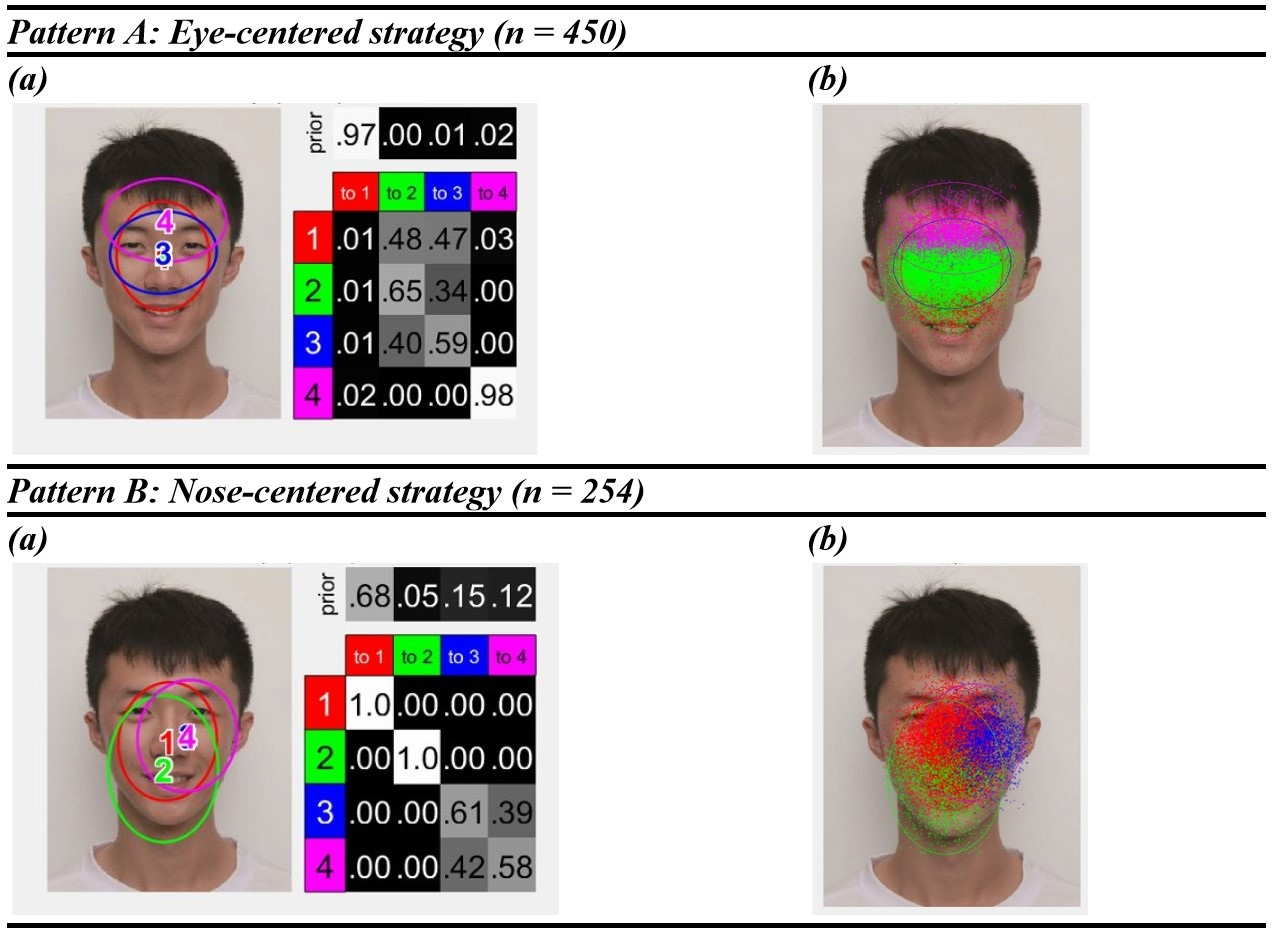
\includegraphics[width=0.7\textwidth]{frog_1.jpg}
\caption*{Notes. (a) The representative hidden Markov model. The ellipses on the left show the ROIs as 2-D Gaussian emissions. The table on the right shows the priors (the probabilities that a fixation sequence starts from the ellipses) and the transition probabilities from one ROI to another in the sequence. (b) The actual assignment of fixations to each ROI.}
\end{figure}


\section{Discussion}
\subsection{Emotion Recognition Performance}
Our collective results showed that individuals with higher social anxiety did not suffer a greater impairment in recognizing masked facial expressions. In our analysis, not only did we fail to find significant interaction effects between social anxiety level and mask use on hit rate, but we also observed that social anxiety was associated with higher hit rates for angry and fearful faces.
Along with a few studies using subclinical samples \citep{SUTTERBY2012242, tibi2011social}, the current results indicate that social anxiety, at subclinical levels, may rather be associated with an enhanced theory of mind, especially for negative emotions. When people with subclinical levels of social anxiety are more sensitive to others’ negative evaluations reflected by facial expressions, they may feel more self-conscious of their behavior during social interactions, causing more anxiety. On the contrary, SAD patients may suffer from an impairment in decoding social signals and experience difficulties in how to respond to them. Indeed, \citet{Nikolić} found a quadratic pattern of the Reading the Mind in the Eyes Test (RMET) performance and SA levels in children: at subclinical levels, social anxiety was associated with better RMET performance, which was mediated by blushing, a physiological marker of heightened self-consciousness. At clinical levels, however, social anxiety was associated with worse RMET performance. Future research should note the potential difference in theory of mind mechanisms underlying social anxiety in the clinical and subclinical populations, and examine it with other paradigms.
\subsection{Eye Movement Patterns}
In addition, our result was also inconsistent with our hypothesis regarding eye movement patterns. We did not find a significant interaction effect between social anxiety levels and mask use, nor did we find a main effect of SA levels on eye movement patterns, suggesting that social anxiety was not associated with a particular eye movement strategy. Therefore, our result is inconsistent with previous studies indicating that high SA individuals tended to avoid direct eye gaze compared with low SA counterparts \citep{horley2003social,weeks2019fear}. The heterogeneous attentional styles within the socially anxious population may explain our failure to uncover the singular eye movement pattern linked to social anxiety. Recent research suggests there may be heterogeneity of threat-related attentional processes among people with high levels of social anxiety. In particular, \citet{Chan16112020} used EMHMM to evaluate the eye movement patterns of healthy college students during free-viewing of neutral and angry faces. Those who consistently adopted either the eye-centered strategy (representing attentional vigilance towards threats) or the nose-centered strategy (representing attentional avoidance), when viewing both facial expressions tended to have higher levels of social anxiety. Hence, two distinct threat-related attentional biases—vigilance and avoidance—may exist among high SA individuals, which may mitigate our efforts to find a uniform eye movement pattern associated with social anxiety in the present study.






\bibliography{references.bib}

\end{document}